%%%%%%%%%%%%%%%%%%%%%%%%%%%%%%%%%%%%%%%%%%%%%%%%%%%%%%%%%%%%%%%%%%%%%%
% Springer LNCS Conference Paper
%%%%%%%%%%%%%%%%%%%%%%%%%%%%%%%%%%%%%%%%%%%%%%%%%%%%%%%%%%%%%%%%%%%%%%

\documentclass[runningheads]{llncs}

\usepackage[T1]{fontenc}
\usepackage{graphicx}
\usepackage{amsmath,amssymb}
\usepackage{booktabs}
\usepackage{multirow}
\usepackage{url}
\usepackage{hyperref}

\begin{document}

\title{Agentic Self-Correction in LLaMA-3: Enhancing E-Commerce Sentiment Analysis through Multi-Agent Reflection}

\titlerunning{Agentic Self-Correction in LLaMA-3 for E-Commerce Sentiment Analysis}

\author{Varun K}

\authorrunning{Varun K}

\institute{
PES University, Bengaluru, India\\
\email{kvarun314@gmail.com}
}

\maketitle

\begin{abstract}

Large Language Models (LLMs) such as LLaMA-3 classify e-commerce review sentiment well, but they act as static, text-only, single-pass classifiers. They cannot verify a reviewer's claims against product facts, they ignore image and metadata evidence, and they are prone to errors on sarcasm and mixed sentiment. This paper presents a multimodal agentic framework that adds verification and reflection on top of a fine-tuned LLaMA-3-8B sentiment classifier. A LoRA-tuned baseline (Phase~1) is wrapped in a four-agent pipeline (Analyst, Visual Verifier, RAG Prover, Critic) with a dissonance-triggered self-correction loop (Phase~2). Both phases are compared on 2\,000 Amazon Reviews 2023 samples (All Beauty category). Phase~2 raises accuracy from 0.161 to 0.387 (+22.6~pp), macro F1 from 0.095 to 0.273, and lowers MAE from 1.52 to 0.96. It recovers 491 Phase~1 errors while introducing 39 new ones, at a 3.7$\times$ latency cost. Most of the gain comes from multimodal context and multi-agent voting; self-correction adds a smaller but measurable benefit on contested samples.

\keywords{
Sentiment Analysis \and
LLaMA-3 \and
LoRA \and
Agentic AI \and
Self-Correction \and
Retrieval Augmented Generation \and
Multimodal Learning
}

\end{abstract}

%%%%%%%%%%%%%%%%%%%%%%%%%%%%%%%%%%%%%%%%%%%%%%%%%%%%%%%%%%%%%%%%%%%%%%
\section{Introduction}
%%%%%%%%%%%%%%%%%%%%%%%%%%%%%%%%%%%%%%%%%%%%%%%%%%%%%%%%%%%%%%%%%%%%%%

Automated Sentiment Analysis (ASA) is central to modern e-commerce, where businesses analyse large volumes of customer feedback to track product quality and user satisfaction. Recent LLMs, particularly LLaMA-3, have improved sentiment classification through strong contextual understanding and reasoning \cite{wang2025}.

However, such models typically run as static, text-only classifiers that produce a prediction in a single inference step without factual verification or reflection. This causes three failure modes. \emph{Sentiment hallucination}: the model treats a user's incorrect claim (e.g.\ ``this watch isn't waterproof'') as a genuine product defect, because it has no access to the specification. \emph{Context blindness}: product images and metadata that could confirm or refute a complaint are ignored. \emph{Linguistic errors}: sarcasm (``Amazing, it broke in two days'') and mixed sentiment are misread, as nothing triggers re-evaluation.

This paper proposes a multimodal agentic framework that does not only \emph{read} sentiment but \emph{verifies} it against product facts and other modalities. The contributions are:
\begin{itemize}
\item A reproduced Phase~1 baseline: LLaMA-3-8B fine-tuned with LoRA on Amazon product reviews.
\item A four-agent pipeline (Analyst, Visual Verifier, RAG Prover, Critic) with a dissonance-triggered self-correction loop.
\item An empirical evaluation on 2\,000 Amazon Reviews 2023 samples with a detailed analysis of \emph{why} the agentic system improves over the baseline.
\end{itemize}

The rest of the paper is organised as follows. Section~2 reviews related work and the research gap. Section~3 describes the datasets. Section~4 presents the baseline and Section~5 the proposed agentic system. Section~6 reports the experimental setup and results, Section~7 analyses them, and Section~8 concludes.

%%%%%%%%%%%%%%%%%%%%%%%%%%%%%%%%%%%%%%%%%%%%%%%%%%%%%%%%%%%%%%%%%%%%%%
\section{Related Work and Research Gap}
%%%%%%%%%%%%%%%%%%%%%%%%%%%%%%%%%%%%%%%%%%%%%%%%%%%%%%%%%%%%%%%%%%%%%%

\textbf{Baseline.} Wang et al.\ \cite{wang2025} fine-tune LLaMA-3-8B with Low-Rank Adaptation (LoRA) \cite{hu2022lora} for product-review sentiment, using TextBlob-based Data Quality Control (DQC), Variant Greedy Search (VGST) for diversity-maximising sampling, and one-shot plus zero-shot chain-of-thought (CoT) prompting. They report 92.6\% accuracy, 95.3\% precision and 93.3\% F1, outperforming SVM and XLNet. Such a model is still a passive, single-pass classifier.

\textbf{Reflection and verification.} Self-RAG \cite{asai2023} trains a model to retrieve, generate and critique through self-reflection, which is analogous to our Critic. MERMAID \cite{mermaid2025} uses a cross-modal verification module for emotion recognition and reports gains of up to 27\% absolute from self-reflection loops, similar to our Visual Verifier. Verifier-in-the-loop guidance \cite{verifier2025} motivates the use of a verifier to prevent hallucination, and LLM agents have also been used as customer simulators for evaluating shopping assistants \cite{sun2025}.

\textbf{Research gap.} Three gaps separate the baseline from our proposal: (i) no \emph{factual grounding}, since user text is assumed correct (``gullibility'' gap); (ii) no \emph{autonomous auditing}, since a lone Analyst cannot catch sarcasm or logical errors (``critic'' gap); and (iii) \emph{modality isolation}, since image evidence that confirms or contradicts a review is ignored (``visual'' gap).

%%%%%%%%%%%%%%%%%%%%%%%%%%%%%%%%%%%%%%%%%%%%%%%%%%%%%%%%%%%%%%%%%%%%%%
\section{Datasets}
%%%%%%%%%%%%%%%%%%%%%%%%%%%%%%%%%%%%%%%%%%%%%%%%%%%%%%%%%%%%%%%%%%%%%%

\textbf{Baseline dataset.} Phase~1 trains on the Kaggle \texttt{arhamrumi/amazon-product-reviews} corpus ($\sim$500\,000 reviews, ratings 1--5). The raw data contains duplicates, inconsistent sentiment--rating pairs and a strong positive bias, which are addressed by DQC and stratified sampling (Section~4).

\textbf{Proposed dataset.} Phase~2 is evaluated on Amazon Reviews 2023 (UCSD McAuley Lab) \cite{hou2024}, which comprises 570 million reviews and 48 million products in 33 categories, with review text, ratings, product metadata (title, description, category, price, specifications) and product images. This enables the multimodal verification that the Kaggle data cannot support. Reviews are loaded as JSONL and metadata as Parquet through the HuggingFace \texttt{datasets} library, without \texttt{trust\_remote\_code}.

\textbf{Disjoint datasets.} Phase~1 (Kaggle) and Phase~2 (Amazon Reviews 2023) use disjoint data. The Phase~1 adapter has therefore never seen the evaluation distribution, and the Phase~1 vs.\ Phase~2 comparison should be read as a generalisation test, not as a same-distribution held-out comparison.

%%%%%%%%%%%%%%%%%%%%%%%%%%%%%%%%%%%%%%%%%%%%%%%%%%%%%%%%%%%%%%%%%%%%%%
\section{Baseline Model (Phase 1)}
%%%%%%%%%%%%%%%%%%%%%%%%%%%%%%%%%%%%%%%%%%%%%%%%%%%%%%%%%%%%%%%%%%%%%%

\textbf{Preprocessing.} Five ordered steps are applied: (1) \emph{TextBlob DQC} drops rows whose polarity contradicts the rating (polarity $<0$ with rating $>3$, or polarity $>0$ with rating $<3$); (2) \emph{stratified sampling} balances counts per rating 1--5, up to 10\,000 rows; (3) \emph{VGST} greedily selects reviews that add the most unseen token IDs when the pool exceeds the target size; (4) \emph{neutral oversampling} duplicates rating-3 rows ($\times2$) to help the hardest class; and (5) the data are shuffled and capped at 4\,000 samples, then split 80/20 into train and validation sets.

\textbf{LoRA fine-tuning.} The LLaMA-3-8B weights are frozen and the update is factorised as
\begin{equation}
h = Wx + \Delta W x = Wx + BAx,
\end{equation}
with $B\in\mathbb{R}^{d\times r}$, $A\in\mathbb{R}^{r\times d}$ and $r\ll d$; $A$ is initialised from a Gaussian and $B=0$, so that $\Delta W=0$ initially. Table~\ref{tbl:lora} compares our configuration with that of Wang et al.\ \cite{wang2025}. Training uses 4-bit NF4 quantisation, gradient checkpointing, and best-checkpoint selection on validation loss. Inference uses one-shot plus CoT prompting with greedy decoding (128 new tokens).

\begin{table}[htbp]
  \centering
\caption{LoRA hyperparameters: Wang et al.\ vs.\ ours}
  \label{tbl:lora}
\small
  \begin{tabular}{lcc}
  \hline
  Parameter & Wang et al. & Ours \\
  \hline \hline
  Learning rate & 5e-5 & 5e-5 \\
  LoRA rank $r$ & 4 & 16 \\
  LoRA alpha $\alpha$ & 64 & 128 \\
  Epochs & 3 & 5 \\
  Batch size / grad.\ accum. & 3 / 4 & 3 / 4 \\
  Target modules & 3 layers & q/k/v/o, 8 layers \\
  Max samples & 2000 & 4000 \\
  Scheduler & cosine & cosine \\
  Compute type & fp16 & 4-bit NF4 + fp16 \\
  \hline
  \end{tabular}
  
\end{table}

\textbf{Phase~1 results.} On 4\,000 held-out Kaggle samples our run reaches $\sim$0.666 accuracy, $\sim$0.684 weighted F1 and $\sim$0.499 macro F1 (Colab T4), against 0.926 accuracy and 0.933 F1 reported by Wang et al. The gap is expected: the baseline paper uses its own larger experimental setup (RTX 4090, different data splits), whereas this work targets sound methodology rather than bit-for-bit reproduction.

On the 2\,000-sample Amazon Reviews 2023 slice (All Beauty), the same adapter reaches only 0.161 accuracy, 0.095 macro F1 and 1.52 MAE. This reflects the transfer to a new distribution and the class imbalance of the slice (1\,181 of 2\,000 samples are 5-star). Phase~2 improvements are measured relative to this figure.

%%%%%%%%%%%%%%%%%%%%%%%%%%%%%%%%%%%%%%%%%%%%%%%%%%%%%%%%%%%%%%%%%%%%%%
\section{Proposed Agentic Framework (Phase 2)}
%%%%%%%%%%%%%%%%%%%%%%%%%%%%%%%%%%%%%%%%%%%%%%%%%%%%%%%%%%%%%%%%%%%%%%

The framework replaces single-pass classification with a stateful multi-agent workflow over review text, product metadata and product images (Figure~\ref{fig:arch}). The LLM used by every agent is the Phase~1 LLaMA-3-8B + LoRA adapter.

\begin{figure}[htbp]
   \centering
    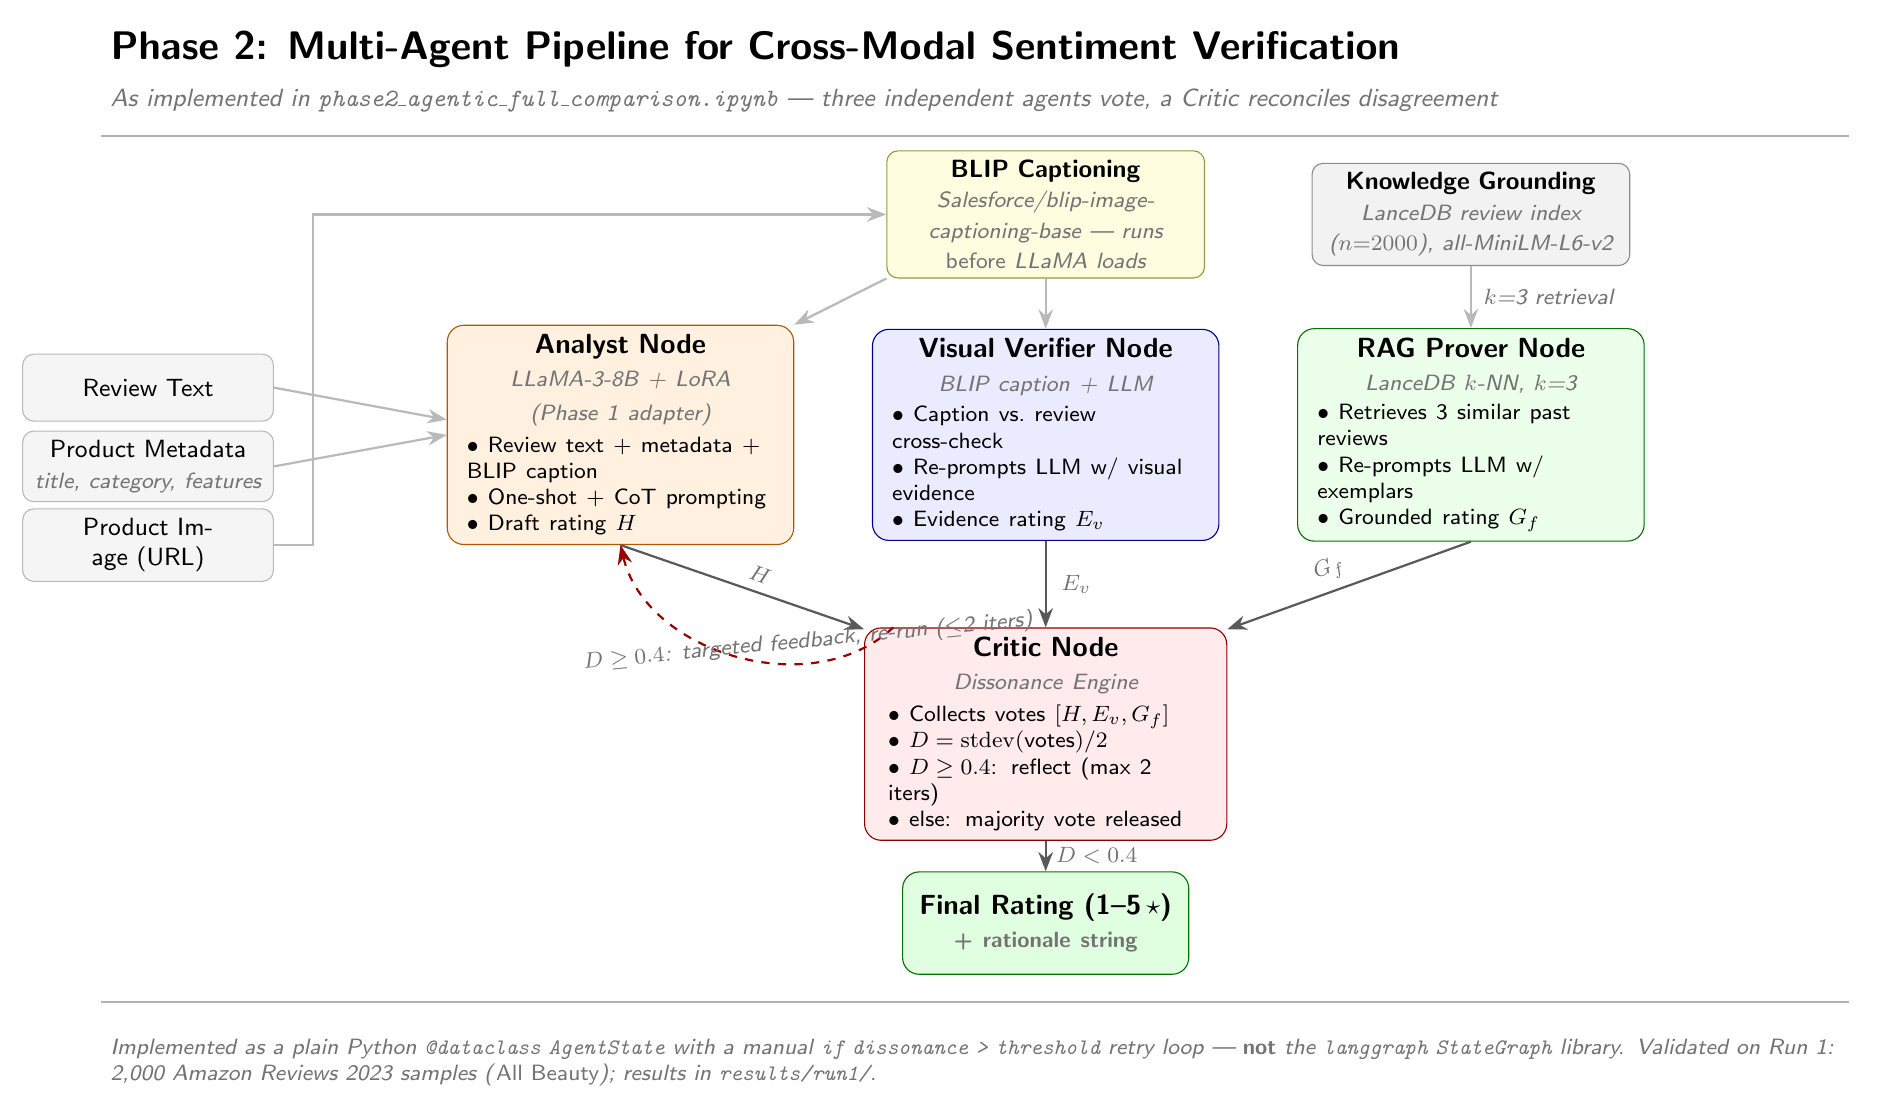
\includegraphics[width=\textwidth]{figures/Phase2_Architecture.png}
   
   \caption{Phase~2 multi-agent architecture. In the executed pipeline, three agents (Analyst, Visual Verifier, RAG Prover) produce independent rating estimates; the Critic computes dissonance $D$ and, if $D\ge0.4$, returns feedback to the Analyst for up to two iterations.}
   \label{fig:arch}
\end{figure}

\textbf{Analyst.} Reads the review text with one-shot plus CoT prompting and produces a preliminary rating, the hypothesis $H$.

\textbf{Visual Verifier.} Downloads the product image and captions it with BLIP (\texttt{Salesforce/blip-image-captioning-base}) \cite{li2022blip}. It re-prompts the LLM with the visual evidence $E_v$ to obtain a second rating.

\textbf{RAG Prover.} Queries a LanceDB vector index (384-d \texttt{all-MiniLM-L6-v2} embeddings of the review corpus) for the $k=3$ nearest exemplars and re-prompts with them to obtain a grounded rating $G_f$.

\textbf{Critic.} Collects the votes $v=[r_{\mathrm{Analyst}}, r_{\mathrm{Visual}}, r_{\mathrm{RAG}}]$ and computes the dissonance
\begin{equation}
D = \frac{\sqrt{\frac{1}{3}\sum_{i=1}^{3}(v_i-\bar v)^2}}{2}.
\end{equation}
If $D<0.4$ the majority vote is released. Otherwise the Critic generates a critique and the Analyst re-runs with this feedback, for at most two iterations.

\textbf{Implementation.} Each sample carries an \texttt{AgentState} record (review, metadata, caption, the four agent ratings, dissonance, correction count, final rating and rationale). BLIP is run before LLaMA is loaded and is then deleted to save VRAM. Results are streamed to a JSONL checkpoint after every sample so that a Colab disconnect does not lose progress. The pipeline is implemented as plain Python functions over this state, with a manual dissonance-triggered retry loop.

%%%%%%%%%%%%%%%%%%%%%%%%%%%%%%%%%%%%%%%%%%%%%%%%%%%%%%%%%%%%%%%%%%%%%%
\section{Experiments and Results}
%%%%%%%%%%%%%%%%%%%%%%%%%%%%%%%%%%%%%%%%%%%%%%%%%%%%%%%%%%%%%%%%%%%%%%

\subsection{Setup}

Table~\ref{tbl:setup} lists the configuration of Run~1. All experiments ran on a Google Colab T4 GPU (16~GB), where the 4-bit LLaMA-3-8B model fits in $\sim$8--10~GB of VRAM.

\begin{table}[htbp]
  \centering
\caption{Experimental configuration (Run 1)}
  \label{tbl:setup}
\small
  \begin{tabular}{ll}
  \hline
  Parameter & Value \\
  \hline \hline
  Dataset & Amazon Reviews 2023, All Beauty \\
  Sample size / seed & 2\,000 / 42 \\
  Model & LLaMA-3-8B + LoRA adapter \\
  Quantisation & 4-bit NF4 \\
  Max new tokens & 128 \\
  Image captioner & BLIP (base) \\
  RAG embeddings & all-MiniLM-L6-v2, $k=3$ \\
  Dissonance threshold & 0.4 \\
  Max correction steps & 2 \\
  Hardware & Google Colab T4 \\
  \hline
  \end{tabular}
  
\end{table}

\subsection{Overall Results}

\begin{table}[htbp]
  \centering
\caption{Phase 1 vs.\ Phase 2, overall metrics (2\,000 samples)}
  \label{tbl:overall}
\small
  \begin{tabular}{lccc}
  \hline
  Metric & Phase 1 & Phase 2 & $\Delta$ \\
  \hline \hline
  Accuracy & 0.1610 & 0.3870 & +22.60 pp \\
  Macro F1 & 0.0946 & 0.2725 & +17.79 pp \\
  MAE & 1.5205 & 0.9635 & $-$0.557 \\
  Mean latency & 0.77 s & 2.83 s & 3.7$\times$ \\
  \hline
  \end{tabular}
  
\end{table}

\begin{figure}[htbp]
   \centering
    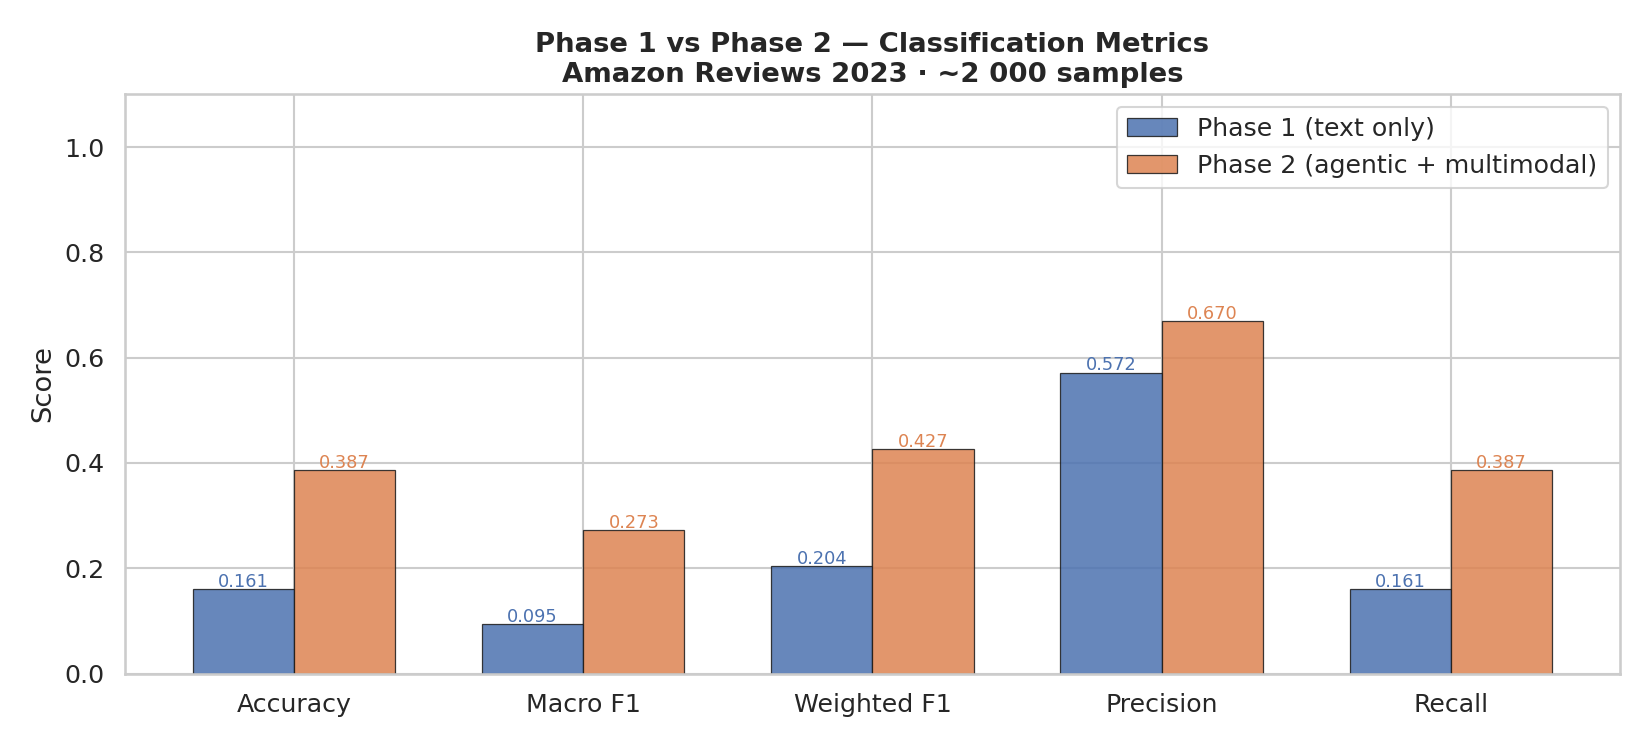
\includegraphics[width=\textwidth]{figures/metrics_comparison.png}
   
   \caption{Phase~1 vs.\ Phase~2 metric comparison on 2\,000 samples.}
   \label{fig:metrics}
\end{figure}

Phase~2 improves accuracy by 22.6~pp, macro F1 by 17.8~pp and reduces MAE by 0.56 (Table~\ref{tbl:overall}, Figure~\ref{fig:metrics}), at 3.7$\times$ the latency. Table~\ref{tbl:perclass} gives per-rating accuracy. The neutral (3-star) class gains most ($+$52.1~pp), because metadata and image context are most useful for disambiguating neutral reviews. The 2-star class shows a slight regression ($-$1.0~pp), a known difficulty for the borderline negative class.

\begin{table}[htbp]
  \centering
\caption{Per-rating accuracy}
  \label{tbl:perclass}
\small
  \begin{tabular}{lcccc}
  \hline
  Rating & $n$ & Phase 1 & Phase 2 & $\Delta$ \\
  \hline \hline
  1$\star$ & 147 & 0.020 & 0.272 & +0.252 \\
  2$\star$ & 105 & 0.019 & 0.010 & $-$0.010 \\
  3$\star$ & 190 & 0.458 & 0.979 & +0.521 \\
  4$\star$ & 377 & 0.000 & 0.053 & +0.053 \\
  5$\star$ & 1181 & 0.195 & 0.446 & +0.251 \\
  \hline
  \end{tabular}
  
\end{table}

\subsection{Error Recovery and Self-Correction}

Phase~2 recovers 491 samples that Phase~1 got wrong and introduces 39 new errors, a net improvement of $+452$ samples and a recovery ratio of 12.6$\times$. The Critic's self-correction was triggered on 922 samples (46.1\%); 669 samples (33.5\%) had $D\ge0.4$. The mean dissonance is 0.211 and the maximum 0.471. The frequent disagreement shows that the ensemble is not trivially redundant.

%%%%%%%%%%%%%%%%%%%%%%%%%%%%%%%%%%%%%%%%%%%%%%%%%%%%%%%%%%%%%%%%%%%%%%
\section{Analysis: Why Phase 2 Works}
%%%%%%%%%%%%%%%%%%%%%%%%%%%%%%%%%%%%%%%%%%%%%%%%%%%%%%%%%%%%%%%%%%%%%%

\textbf{Rating collapse in Phase 1.} Phase~1 collapses to a narrow range of predictions (Table~\ref{tbl:dist}). It predicts 4-star only 25 times despite 377 true 4-star samples, over-predicts 3-star by 6.6$\times$, and 90.2\% of its errors are under-predictions. Phase~2 distributes predictions more faithfully; its 5-star predictions rise from 241 to 569.

\begin{table}[htbp]
  \centering
\caption{Prediction distribution vs.\ ground truth}
  \label{tbl:dist}
\small
  \begin{tabular}{lccccc}
  \hline
   & 1$\star$ & 2$\star$ & 3$\star$ & 4$\star$ & 5$\star$ \\
  \hline \hline
  Ground truth & 147 & 105 & 190 & 377 & 1181 \\
  Phase 1 & 349 & 124 & 1261 & 25 & 241 \\
  Phase 2 & 51 & 10 & 1289 & 81 & 569 \\
  \hline
  \end{tabular}
  
\end{table}

\textbf{Where recoveries come from.} Nearly 80\% of the 491 recoveries come from two transitions: Phase~1 predicts 3-star and Phase~2 corrects to 5-star (288, 58.7\%), and 1-star corrected to 3-star (100, 20.4\%). An ambiguous review becomes clearly positive once the Visual Verifier sees a clean product image and the RAG Prover retrieves highly rated similar reviews.

\textbf{Agent specialisation.} On the 774 samples that Phase~2 classifies correctly, the Visual Verifier's vote matches the ground truth in 97.7\% of cases, the RAG Prover's in 91.2\%, and the Analyst's in only 64.9\% (Table~\ref{tbl:agents}). The ensemble thus overrules the conservative text-only Analyst on 35\% of its correct predictions, and the two context-aware agents systematically push the vote towards the true rating.

\begin{table}[htbp]
  \centering
\caption{Per-agent vote alignment on Phase~2-correct samples ($n=774$)}
  \label{tbl:agents}
\small
  \begin{tabular}{lcc}
  \hline
  Agent & Correct votes & Rate \\
  \hline \hline
  Analyst (text only) & 502 / 774 & 64.9\% \\
  RAG Prover & 706 / 774 & 91.2\% \\
  Visual Verifier & 756 / 774 & 97.7\% \\
  \hline
  \end{tabular}
  
\end{table}

\textbf{Dissonance as a proxy for difficulty.} Table~\ref{tbl:diss} groups samples by dissonance. Even when the agents fully agree ($D<0.1$), Phase~2 is 23.9~pp better than Phase~1, so the gain does not come primarily from self-correction but from the additional context. Gains are largest under moderate disagreement ($+$36.0~pp) and smallest for high dissonance ($+$11.7~pp), which are the genuinely hardest samples.

\begin{table}[htbp]
  \centering
\caption{Accuracy by dissonance level}
  \label{tbl:diss}
\small
  \begin{tabular}{lccc}
  \hline
  Dissonance $D$ & $n$ & Phase 1 & Phase 2 \\
  \hline \hline
  $[0.0, 0.1)$ & 867 & 0.241 & 0.480 \\
  $[0.2, 0.3)$ & 464 & 0.078 & 0.438 \\
  $[0.4, 1.0)$ & 669 & 0.115 & 0.232 \\
  \hline
  \end{tabular}
  
\end{table}

\textbf{Self-correction is useful but secondary.} On the 922 samples where self-correction ran, Phase~1 accuracy is 0.095 and Phase~2 accuracy is 0.261 ($+$16.6~pp). On the remaining samples Phase~2 gains $+$27.7~pp. Context enrichment is therefore the primary driver, multi-agent majority voting the second, and self-correction on genuinely ambiguous reviews the third.

%%%%%%%%%%%%%%%%%%%%%%%%%%%%%%%%%%%%%%%%%%%%%%%%%%%%%%%%%%%%%%%%%%%%%%
\section{Discussion}
%%%%%%%%%%%%%%%%%%%%%%%%%%%%%%%%%%%%%%%%%%%%%%%%%%%%%%%%%%%%%%%%%%%%%%

\textbf{Benefits.} Richer context helps borderline ratings the most; multi-agent specialisation is more robust than any single agent; and explainability is structural, since Phase~2 yields a per-agent vote, a dissonance score, a correction trace and a rationale, where Phase~1 yields an opaque single output. The 12.6$\times$ recovery ratio shows that corrections are almost always beneficial.

\textbf{Limitations.}
(i) Absolute accuracy (38.7\%) remains low because the slice is heavily skewed to 5-star reviews; a balanced test set would likely give higher figures.
(ii) BLIP captions depend on image availability and quality.
(iii) The RAG index holds review embeddings, not product specifications, so the Prover retrieves similar reviews and does not check claims against a specification store.
(iv) The 3.7$\times$ latency overhead suits offline batch analysis but not real-time use.
(v) The Phase~1 adapter is trained on a different dataset from the one evaluated.

%%%%%%%%%%%%%%%%%%%%%%%%%%%%%%%%%%%%%%%%%%%%%%%%%%%%%%%%%%%%%%%%%%%%%%
\section{Conclusion}
%%%%%%%%%%%%%%%%%%%%%%%%%%%%%%%%%%%%%%%%%%%%%%%%%%%%%%%%%%%%%%%%%%%%%%

A four-agent framework with dissonance-triggered self-correction improves LLaMA-3 sentiment classification on 2\,000 Amazon Reviews 2023 samples from 16.1\% to 38.7\% accuracy, with a 12.6$\times$ ratio of recovered to introduced errors. Analysis shows the gain comes mainly from multimodal context and multi-agent voting, and secondarily from self-correction. Future work includes a production vector store with CLIP-indexed product specifications, a vision-language Analyst (e.g.\ LLaVA-class) for direct image understanding, deeper multi-round reflection at scale, and comparison with classical baselines (Decision Tree, SVM, XLNet) on the Amazon 2023 slice.


\subsubsection*{Acknowledgements.} This work was carried out as part of an M.Tech project at PES University. Code, results and the trained LoRA adapter: \url{https://github.com/kvarun314/pes-mtech-project}.

\begin{thebibliography}{8}

\bibitem{wang2025}
Wang, et al.: Sentiment Analysis of Product Reviews Using Fine-Tuned LLaMa-3 Model. ITM Web of Conferences 70, 04021 (2025)

\bibitem{asai2023}
Asai, A., Wu, Z., Wang, Y., Sil, A., Hajishirzi, H.: Self-RAG: Learning to Retrieve, Generate, and Critique through Self-Reflection. arXiv:2310.11511 (2023)

\bibitem{mermaid2025}
MERMAID: Multi-perspective Self-reflective Agents with Generative Augmentation for Emotion Recognition. In: Proc. EMNLP 2025, ACL Anthology 2025.emnlp-main.1252 (2025)

\bibitem{verifier2025}
Local Look-Ahead Guidance via Verifier-in-the-Loop for Automated Theorem Proving. arXiv:2503.09730 (2025)

\bibitem{sun2025}
Sun, et al.: Can LLM Agents Simulate Customers to Evaluate Agentic-AI-based Shopping Assistants? arXiv:2509.21501 (2025)

\bibitem{hou2024}
Hou, Y., Li, J., He, Z., Yan, A., Chen, X., McAuley, J.: Bridging Language and Items for Retrieval and Recommendation. arXiv:2403.03952 (2024)

\bibitem{hu2022lora}
Hu, E.J., et al.: LoRA: Low-Rank Adaptation of Large Language Models. In: ICLR (2022)

\bibitem{li2022blip}
Li, J., Li, D., Xiong, C., Hoi, S.: BLIP: Bootstrapping Language-Image Pre-training for Unified Vision-Language Understanding and Generation. In: ICML (2022)

\end{thebibliography}

\end{document}
